
\chapter{Conclusions and perspectives} \label{summmary}
\graphicspath{{chapter7_ys/}}


\section{Conclusions and discussion}

In this PhD thesis, a robust reflectometry spectrum parametrization method has been developed for systematic studies of turbulence properties in fusion plasmas. Equipped with a routinely applicable spectrum parametrization technique, we have been able to study trends of several spectrum characteristics that occur robustly throughout significant parts of the database. Some of these patterns were only revealed with the availability of large data sets spanning a wide range of plasma conditions. In turn, a physical interpretation for the observed patterns has been proposed in terms of a transition between the dominant instability driving the turbulence. This interpretation may be compatible with earlier simulations and experiments performed on a limited set of discharges. Our work has allowed, for the first time in fusion science, to systematically characterize trends of fluctuation properties over a large database. This large-scale approach is complementary to the traditional analysis methods on the basis of a limited number of key discharges. Our work is intended to open the way to a new, standardized method for studying plasma density fluctuations ($\delta n$) from a systematic viewpoint.

The spectrum parametrization method has been developed using a large database with 350,000 frequency spectra obtained from Tore Supra plasmas. The method is also useful for quantifying the power spectrum in individual discharges, and can be easily adapted to other fusion devices or other research domains relying on quantitative comparison of spectra. The main contribution of the technique is that it allows quantification of spectra in a standardized way, enabling comparison across experimental conditions and devices. In fitting the spectra with a reduced model, the generalized Gaussian, Voigt, and Taylor distributions have been used to parameterize the various components of the fluctuation power spectra. Both the generalized Gaussian and the Taylor models yield excellent performance in terms of goodness-of-fit, while meeting the requirements of flexibility, discrimination, and robustness. The Taylor model is a more convenient model with a view to physical interpretation. In implementing the fitting routine, the cost function, the constraints and the initial guesses have been identified as critical points. The cost function consists of equally weighted components on the linear and logarithmic scale, imposing several constraints on the parameters in order to separate the different spectrum components.

Full radial profiles of the broadband (BB) contribution ($E_\mathrm{BB}$) of the frequency spectra have been studied for different edge safety factors ($q_{\psi}$). In Ohmic plasmas, an remarkable drop of $E_\mathrm{BB}$, called the $E_\mathrm{BB}$ basin, was systematically observed inside the $q = 1$ surface. The basin width is clearly linked to the position of the $q = 1$ magnetic surface. Outside the $q = 1$ surface at both the high-field-side (HFS) and low-field-side (LFS), $E_\mathrm{BB}$ reaches a high magnitude ($E_\mathrm{BB} > 0.5$) but a strong asymmetry occurs of the $E_\mathrm{BB}$ trend with radius
at the HFS vs. the LFS. In addition, a systematic shift of the cutoff layers to the HFS is probably caused by underestimation of the electron density in the core region by the interferometry diagnostic. Furthermore, similar trends were recovered when discriminating between the linear confinement regime (LOC) and the saturated confinement regime (SOC). However, $E_\mathrm{BB}$ was observed to be systematically higher in the SOC regime, compared to the LOC regime. In L-mode plasmas, with auxiliary ICRH or LH heating, $E_\mathrm{BB}$ with pure LH heating remains at almost the same level as in Ohmic plasmas, and only a small increase of $E_\mathrm{BB}$ could be observed with increasing power. In contrast, with ICRH heating, $E_\mathrm{BB}$ was significantly higher than in the Ohmic case, even at low heating power, saturating at high heating power. The $E_\mathrm{BB}$ basin in the core region is very shallow or even non-existent with ICRH heating. Moreover, increasing $q_{\psi}$ generally causes a small increase of $E_\mathrm{BB}$ for both ICRH and LH plasmas.

The global trends of the $E_\mathrm{BB}$ profiles observed in both the Ohmic and L-mode plasmas agree with results from the literature regarding the behavior of density fluctuations in various confinement regimes. Our work has extended the validity of these results to a much wider range of plasma conditions. Indeed, $E_\mathrm{BB}$ is possibly proportional to the density fluctuation level when it is small ($E_\mathrm{BB} < 0.5$), whereas this linear relation becomes invalid at larger $E_\mathrm{BB}$. A correction of $E_\mathrm{BB}$ considering the density gradient length and the frequency of the probing waves may provide a more accurate estimate for the density fluctuation level, but doing this for the whole database is infeasible.

The effective collisionality ($\nu_\mathrm{eff}$) has been found to have a crucial impact on the various components of the frequency spectra. For the BB component, a general increasing trend of $E_\mathrm{BB}$ with respect to $\nu_\mathrm{eff}$ has been observed at different radial positions for both Ohmic and L-mode plasmas. The general trends of the BB width ($W_\mathrm{BB}$) and shape ($\beta_\mathrm{BB}$) are usually more difficult to extract, except for $W_\mathrm{BB}$ in L-mode plasmas, where an increase of $W_\mathrm{BB}$ with $\nu_\mathrm{eff}$ was observed systematically across the radius. The pattern of $\beta_\mathrm{BB}$ is similar for Ohmic and L-mode plasmas. Usually, the dispersion of the data becomes strongest at a moderate $\nu_\mathrm{eff}$ and $\beta_\mathrm{BB}$ tends to converge to the value of 1 (heavy-tailed Laplacian) at high $\nu_\mathrm{eff}$. Regarding the low-frequency (LF) component, a weakly increasing trend of the LF width ($W_\mathrm{LF}$) was observed at the HFS and at the center for both Ohmic and L-mode plasmas.

The observed dependence of $E_\mathrm{BB}$ on $\nu_\mathrm{eff}$ indicates a possible link between the spectrum and the underlying instability driving the turbulence. This assumption was supported by earlier GENE simulations, showing much wider BB and LF components in the SOC regime, with a reduced TEM instability. The systematic trend in $W_\mathrm{LF}$ supports this interpretation, together with our analysis of the density peaking. For both Ohmic and L-mode plasmas, density peaking increases with $\nu_\mathrm{eff}$ at low $\nu_\mathrm{eff}$ and decreases at high $\nu_\mathrm{eff}$. Thus, the observed trends seem to be compatible with a transition of the dominating instability from TEM to ITG.

A useful byproduct of our database approach is the ability to detect faults in diagnostics, possibly indicated by off-normal clusters or trends, or outliers in the database. Other unusual patterns might be due to specific experimental conditions, but may also point at interesting physics, to be explored in a more detailed analysis on a limited data set.

Concluding, the systematic trends observed in this PhD work confirm the relevance of the database approach. Ongoing developments in artificial intelligence are rapidly impacting a broad variety of scientific domains. Likewise, in fusion science, such developments may well lead researchers to new discoveries and a deeper understanding of the fusion plasma.


\section{Perspectives}


Since this thesis is the first systematic analysis of complicated turbulence measurements in fusion study, it has opened windows for many research directions. We now discuss perspectives to future work, following the achievements described in the present thesis.

\subsection*{Extension of this thesis}

Tore Supra operated until 2011, when the transition to the new WEST tokamak was started. In WEST, the poloidal cross-section of the plasma was changed to the more modern D-shape, as shown in figure \ref{fig:ts2west}. Equipped with a new divertor and with auxiliary ICRH and LH heating, realisation of the H-mode is anticipated. The new plasma shape and parameters make it possible to carry out a systematic comparison of turbulence properties between Tore Supra and WEST. Because in WEST the magnetic ripple in the edge has been reduced to much lower levels compared to Tore Supra, it may become possible to extend the spectral analysis to the edge region. Furthermore, it is possible to extend the study to Doppler reflectometer, other diagnostic systems, or even other devices with proper adaption. In addition, influence of the instrumental configuration like the radiation pattern of antennas can also be investigated.



%%%%%%%%%%%%%%%%%%%%
\begin{figure}[h]
\begin{centering}
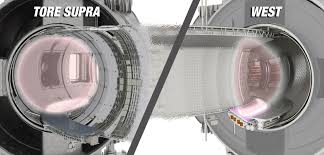
\includegraphics[scale=0.6]{ts2west.jpg}
\par\end{centering}
\caption{From the circular cross-section limiter Tore Supra to the D-shape cross-section divertor WEST (Tungsten (W) Environment in Steady-state Tokamak).}
\label{fig:ts2west}
\end{figure}
%%%%%%%%%%%%%%%%%%%%


\subsection*{Data analysis capabilities}

There are also many ways in which the data analysis techniques applied in the present study could be improved. The strong dispersion of the data suggest that additional plasma parameters may have to be employed to better order the data and characterize trends of the fluctuation spectra. On the other hand, while the individual parameters used to characterize each spectrum may be interpreted from a physical point of view, each of them only quantifies a certain aspect of the spectrum. Modern data science has developed techniques for quantifying distributions and shapes in a more integrated way \cite{Shabbir_2016_RSI}. Combined with specialized similarity measures between shapes or distributions, a more faithful comparison between spectra would become feasible. In turn, this could also contribute to more significant patterns in the data.


\subsection*{Additional spectrum components}

As mentioned in Chapter \ref{ch:Parametrization}, to focus on the most important characteristics of the frequency spectra, only the most common components (DC, LF, BB and N) have been considered in the parametrization. Neglecting other components with narrow bandwidth does not affect the reported general trends of the identified components. However, it might be envisaged to add more parameters to enable capturing also other components, notably the QC modes. This might help to strengthen the link between the spectra and the dominating micro-instabilities, and to explore additional physical properties of the turbulent fluctuations. Specifically, the QC modes could be fitted by another Gaussian functions, with different amplitude for the negative and positive QC modes. Combined with the GG or Taylor model developed in Chapter \ref{ch:Parametrization}, the improved model would include 15 parameters to characterize the spectra with QC modes, as shown in figure \ref{fig:QC_fit}.

%%%%%%%%%%%%%%%%%%%%
\begin{figure}[h]
\begin{centering}
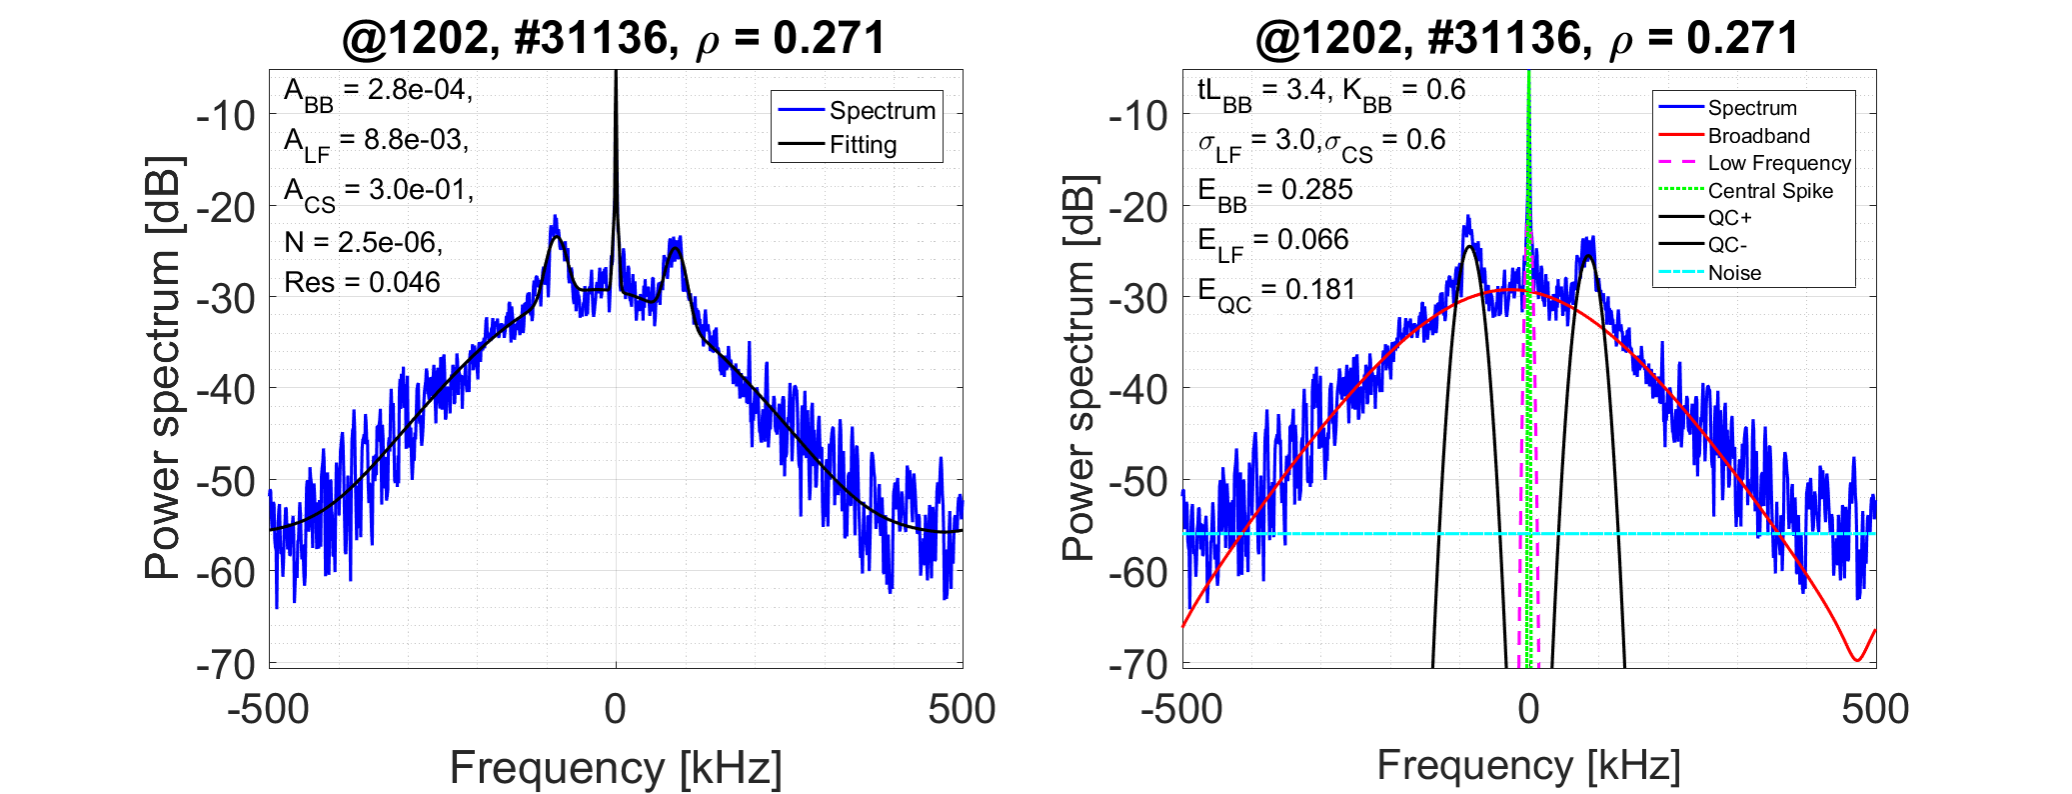
\includegraphics[scale=0.4]{fig_QC_fit.png}
\par\end{centering}
\caption{Include another 4 parameters to fit the quasi-coherent (QC) mode in spectra.}
\label{fig:QC_fit}
\end{figure}
%%%%%%%%%%%%%%%%%%%%

With the increased number of parameters, the problem of misfit or overfit might become more severe, especially when the amplitude of the QC modes is weak compared to the BB component and thus are difficult to be detected. Therefore, a robust fitting algorithm would need to include appropriate constraints on the fit parameters. Another approach could be to dynamically adapt the number of parameters (or functions) according to the spectral characteristics. Here as well, machine learning techniques could make a valuable contribution by clustering the spectra with QC modes into different categorise according to the intensity of the QC modes.


\subsection*{Application to coherence spectra}

In this thesis only the parametrization of the power spectra has been discussed. The coherence spectra from radial or poloidal correlation measurements could provide more spatial and temporal characteristics of turbulent eddies, which cannot be obtained from the power spectra. The features and components of coherence spectra could in general be different from those of power spectra. In tokamak plasmas, the uncorrelated BB component could disappear in coherence spectra. In addition, the LF component could also disappear in long-range correlation analysis \cite{Kramer-Flecken_2015_NJP}. Therefore, when fitting the different components of the coherence spectra with parameterized functions, the number of functions should be adapted depending on experimental conditions.
